\documentclass{article}
\usepackage[utf8]{inputenc}
\usepackage[english, russian]{babel}
\usepackage{graphicx}
\usepackage[hcentering, bindingoffset = 10mm, right = 15 mm, left = 10 mm, top=20 mm, bottom = 20 mm]{geometry}
\DeclareGraphicsExtensions{.pdf,.png,.jpg}
\usepackage{tikz}
\usepackage{amsmath,amsfonts,amssymb,amsthm,mathtools}
\usepackage{multirow}
\usepackage{lipsum}
\usepackage{amsmath, amstext}
\usepackage{siunitx}
\usepackage{subcaption}
\usepackage{ upgreek }
\usepackage{wrapfig}
\usepackage{adjustbox}
\usepackage{enumerate, indentfirst, float}
\usepackage{capt-of, svg}
\usepackage{icomma}
\usepackage{amsmath}
\usepackage{ amssymb }
\usepackage{mathrsfs}
\usepackage{hyperref}
\usepackage{ gensymb }
\usepackage{graphicx}
\graphicspath{{pictures/}}
\DeclareGraphicsExtensions{.pdf,.png,.jpg}
\usepackage{amssymb}
\usepackage{pgfplots}
\usepackage{multirow}
\usepackage{gensymb} 
\usepackage{color}
\usepackage{dsfont}
\usepackage{setspace}

\title{Проект по предмету "Введение в финансы"}
\author{\\}

\begin{document}

    \maketitle
    \thispagestyle{empty}
	\begin{center}
		\rule{\linewidth}{0.5mm} \\[0.4cm]
	{ \Huge\bfseries Модель связи реального эффективного обменного курса рубля и цены на нефть\\  [0.4cm] }
		\rule{\linewidth}{0.5mm} \\[0.4cm]
	\end{center}	
	
    \begin{minipage}{0.6\textwidth}
	\begin{flushleft} \large
		\emph{Автор:}\\
		Востриков Даниил
	\end{flushleft}
\end{minipage}


\newpage 

\section{Аннотация}
В работе предлагается линейная модель связи реального эффективного обменного  курса рубля(\textbf{reer})  и цены на нефть(была выбрана марка Brent, будем обозначать \textbf{poil}), учитывающая наличие изменения денежно-кредитной политики Банка России(далее ДКП) в ноябре 2014 года, а затем и в феврале 2017 года. Показано, что !!! дописать !!!!
\section{Введение}
Обменный курс рубля, пожалуй, является самой обсуждаемой макроэкономической переменной в России. Его величина определяет покупательную способность населения, конкурентоспособность отечественного производства на внутреннем и на внешнем рынке, стоимость импортных товаров промежуточного и инвестиционного назначения, издержки, сопряженные с выплатами внешнего долга.

Важной особенностью российской макроэкономической динамики является частое изменение режимов экономической политики, что сильно осложняет задачу построения эконометрических моделей для прогнозирования и структурного анализа. Наиболее ярким примером таких изменений является смена режимов денежно‐кредитной политики Банка России и, в частности, политики в области курсообразования. После кризиса 1998 г. и до 2003 г. включительно ЦБ управлял денежной базой и краткосрочными колебаниями обменного курса. В период бурного роста нефтяных цен 2004–2008 гг. Банк России активно накапливал валютные резервы, что сопровождалось созданием в 2004 г. стабилизационного фонда и абсорбированием поступающей в бюджет в виде налогов части выручки от экспорта нефти. В рамках проводимой экономической политики номинальный обменный курс рубля был фактически привязан к бивалютной корзине. Во время кризиса 2008–2009 гг. Банк России допустил плавную девальвацию рубля в ответ на ухудшение внешнеэкономических условий и до конца 2014 г. управлял одновременно краткосрочными колебаниями обменного курса и процентными ставками. В конце 2014 г. ЦБ полностью перешел к режиму плавающего обменного курса и таргетирования инфляции. А в феврале 2017 года Минфин России начал ежемесячно покупать иностранную валюту в объеме превышения фактических поступлений нефтегазовых доходов над уровнем нефтегазовых доходов федерального бюджета, сформированного при цене 40 долл. США за баррель нефти марки «Юралс». Все эти изменения в политике курсообразования рубля можно легко проследить на \textbf{рис. 1}, где представлен временной ряд номинального эффективного обменного курса рубля.

\begin{center}
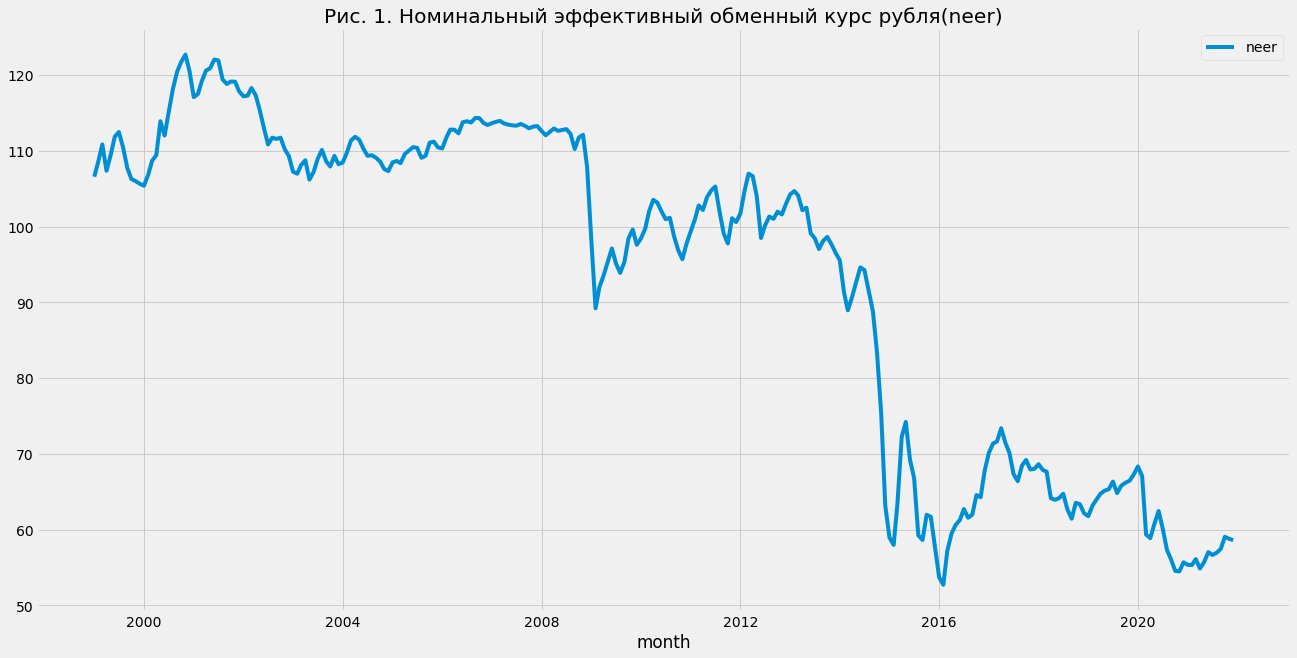
\includegraphics[width=150mm]{neer.png}
\end{center}

\textbf{Опр. 1.} Номинальный эффективный обменный курс (\textbf{neer}) представляет собой взвешенный индекс номинальных обменных курсов местной валюты в пересчете на иностранную валюту. Проще говоря, это можно понимать как конкретную сумму в местной валюте, необходимую для покупки иностранной валюты. NEER указывает на конкурентоспособность страны на валютном рынке (FOREX) и часто упоминается трейдерами ФОРЕКС как индекс торгуемой валюты. Номинальный эффективный обменный курс (\textbf{neer}) не определяется отдельно для каждой страны, этот индекс просто показывает стоимость национальной валюты относительно нескольких иностранных валют. Экономики также корректируют NEER для контроля инфляции в стране. \textbf{neer} валюты растет, когда стоимость национальной валюты увеличивается по отношению к другим иностранным валютам в том же режиме, в то время как, когда ее стоимость падает, \textbf{neer} обесценивается.

\textbf{Опр. 2.} Как и \textbf{neer}, реальный эффективный обменный курс (\textbf{reer}) представляет собой взвешенный индекс цен, который показывает средневзвешенное значение валюты по основным валютам в корзине. \textbf{reer} указывает на конкурентоспособность национальной валюты по отношению к основным валютам международной торговли. \textbf{reer} можно просто определить по относительному торговому балансу национальной валюты с другими валютами в корзине. Увеличение \textbf{reer} указывает на то, что страна теряет свою конкурентоспособность в международной торговле, поскольку ее экспорт дорожает, а импорт дешевеет.

Мы концентрируем внимание на реальном обменном курсе рубля, а не на номинальном, потому что именно этот показатель характеризует конкурентоспособность российской экономики. На \textbf{рис.2} можно видеть уже совместные графики для временных рядов \textbf{reer} и \textbf{poil}. Как видно из графиков, зависимость между величинами действительно есть. Давайте разберемся почему, рассмотрев кратко предпосылки взаимосвязи реального обменного курса с возможными долгосрочными его детерминантами. При анализе детерминант реального курса рубля в качестве прокси переменной для условий торговли России обычно используются цены на нефть в связи с превалирующей долей углеводородов в совокупном экспорте РФ. Улучшение условий торговли (в частности, увеличение нефтяных цен) означает, что за тот же объем экспортируемых товаров отечественная экономика может позволить себе приобрести больший объем импортных товаров, то есть в определенном смысле происходит трансферт богатства отечественной экономике со стороны внешнего мира. От увеличения богатства происходит увеличение спроса и на импортные товары, и на отечественные. В рамках предположения о малой открытой экономике кривая предложения импортных товаров будет горизонтальной (по оси абсцисс – физические объемы, по оси ординат – цены), а кривая предложения отечественных товаров в связи с ограниченностью трудовых ресурсов будет либо вертикальна, либо будет иметь положительный наклон. Таким образом, увеличение агрегированного спроса должно транслироваться в увеличение импортируемой продукции и в увеличение цен на отечественные товары, сопровождающееся, возможно, увеличением их объема производства. Другими словами, при наличии равновесия на внутреннем товарном рынке, чтобы обеспечить выполнение внешнего равновесия в долгосрочном периоде, отечественные экономические агенты должны потреблять больше импортных товаров по отношению к отечественным товарам, для чего отечественные товары должны стать относительно дороже импортных, то есть реальный курс рубля должен укрепиться.

\begin{center}
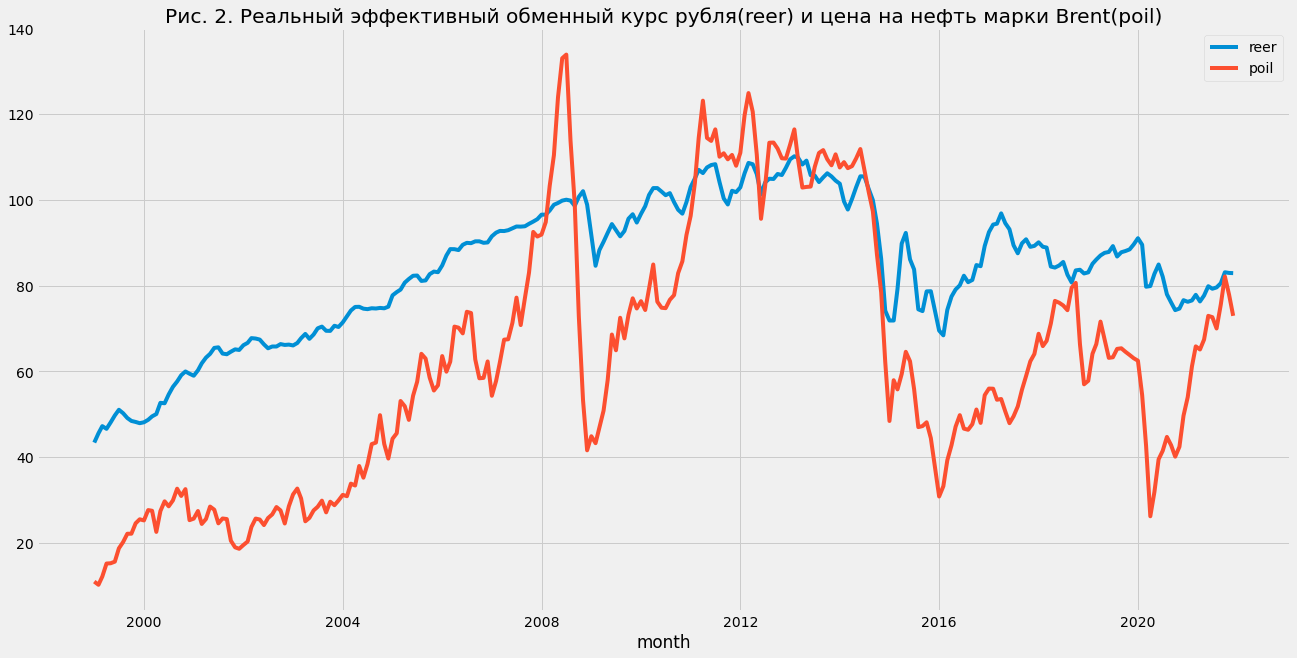
\includegraphics[width=150mm]{reer_poil.png}
\end{center}
\section{Теория по коинтегрированным временным рядам}
Пусть $y_t\sim I(1)$,  $x_t\sim I(0)$. Строить регрессию $y_t$ на $x_t$ в этом случае бессмысленно, т.к. для любых $a$ и $b$ в такой ситуации
$$y_t-a-bx_t\sim I(1).$$
Пусть, наоборот, $y_t \sim I(0)$, $x_t \sim I(1)$. Для любых $a$ и $b \neq 0$ здесь опять 
$$y_t-a-bx_t\sim I(1),$$
и только при $b = 0$ получаем
$$y_t-a-bx_t \sim I(0),$$
так что и в таком сочетании строить регрессию одного ряда на другой не имеет смысла.

Пусть теперь $y_t \sim I(1)$, $x_t \sim I(1)$ – два интегрированных ряда.
Если для любого b
$$y_t-a-bx_t\sim I(1),$$
то регрессия $y_t$ на $x_t$ является \textbf{фиктивной}.

Обратимся теперь к случаю, когда при некотором $b \neq 0$
$$y_t - b x_t \sim I(0)$$ 
-- стационарный ряд. Если это так, то ряды $y_t$ и $x_t$ называют \textbf{коинтегрированными} рядами, а вектор $(1, -b)^T$ -- \textbf{коинтегрирующим} вектором.

Знаменитый результат Гренджера ([Granger (1983)], см. также [Engle, Granger (1987)]), состоит в том, что в случае коинтегрированности $I(1)$ рядов $x_t$ и $y_t$ имеет место так называемая \textbf{модель коррекции ошибок(ECM)}:
$$\Delta y_t=c_1+c_2z_{t-1}+\sum_{i=0}^p{a_i \Delta x_{t-i}}+\sum_{j=1}^q{b_i \Delta y_{t-j}}+\varepsilon_t,~~(!!)$$
где $z_t=y_t-bx_t-E(y_t-bx_t)$ -- стационарный ряд с нулевым матожиданием. В формуле (!!) часть $(c_1+c_2z_{t-1})$ -- отклонение от долгосрочной связи, $r$ и $p$ -- кол-во запаздывающих разностей.

\section{Данные}
Эмпирический анализ в работе проводится на месячных данных за период с января 1999 г. по декабрь 2021 г. При выборе левого конца временного отрезка было принято решение исключить нестабильный период трансформационного спада российской экономики. Выбор правого конца временного отрезка обусловлен наличием статистических данных на момент написания статьи. В расчетах используются следующие временные ряды:
\begin{enumerate}
\item $log(reer_t)$ — натуральный логарифм реального эффективного обменного курса рубля (источник данных: IMF);
\item $log(poil_t)$ — логарифм цены на нефть марки Brent(источник данных: \url{https://worldtable.info/yekonomika/cena-na-neft-marki-brent-tablica-s-1986-po-20.html?ysclid=l9e4pvjjpm293058322}).
\end{enumerate}
На \textbf{рис. 3.} изображен график совместного распределения временных рядов $log(reer_t)$ и  $log(poil_t)$ с линейной аппроксимации. Из графика видно, что временные ряды действительно коинтегрированы, но это еще предстоит выяснить. 

\begin{center}
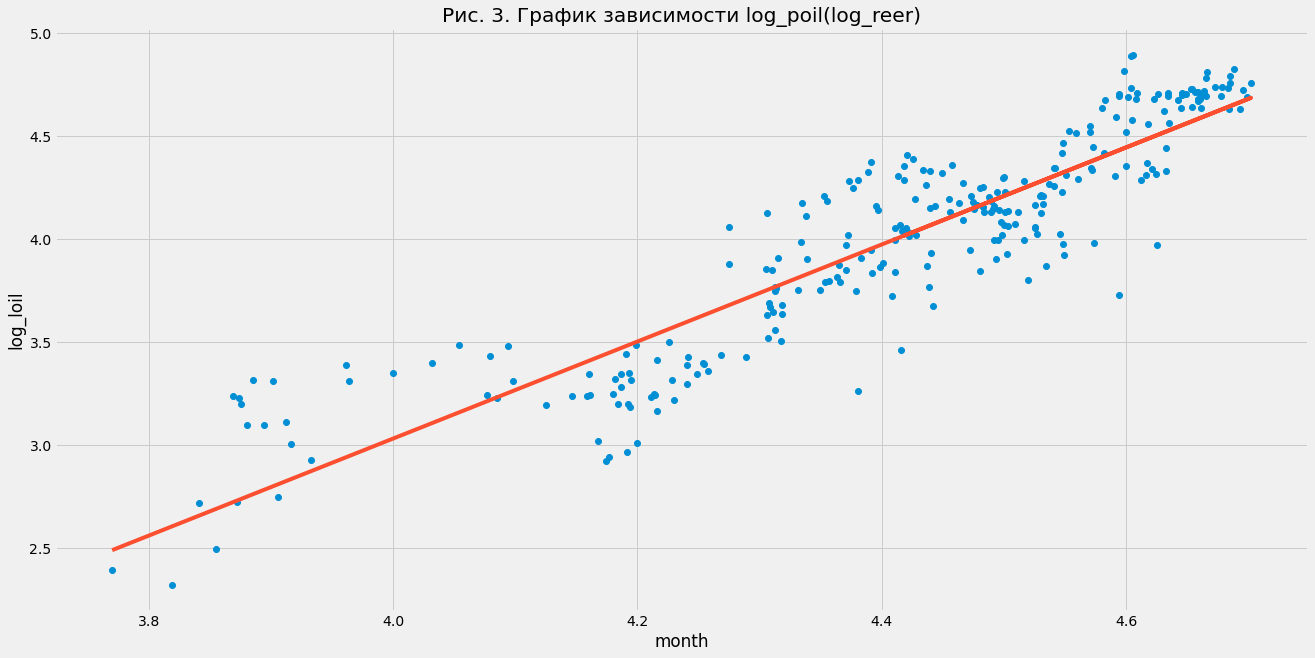
\includegraphics[width=150mm]{log_reer_log_poil.png}
\end{center}

\section{Эмпирический анализ}
\subsection{}
Вначале мы проверим гипотезу о том, что реальный эффективный обменный курс рубля и цена на нефть марки Brent имеют единичный корень:
$$reer_t\sim I(1),~poil_t\sim I(1).$$
Для этого воспользуемся ADF-тестом.
\begin{enumerate}
\item ADF-тест на стационарность ряда $reer_t$:
\begin{center}
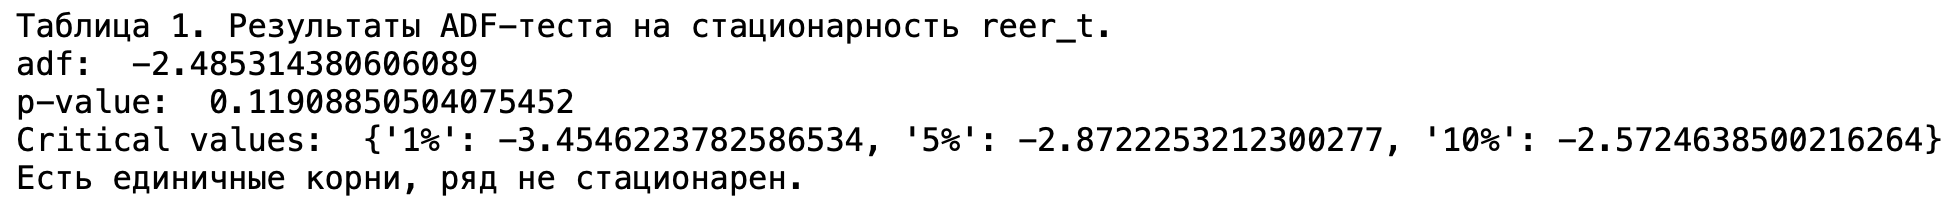
\includegraphics[width=150mm]{table_adf_reer.png}
\end{center}

\item ADF-тест на стационарность продифференциированного ряда 
$\Delta reer_t$:
\begin{center}
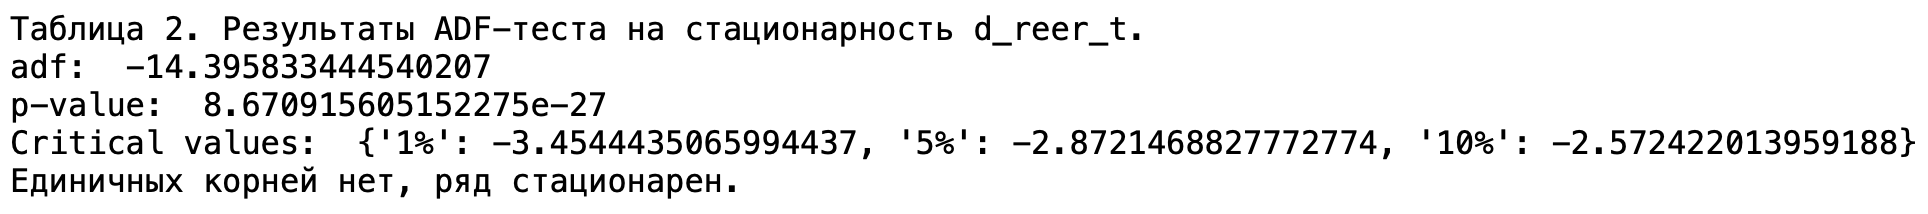
\includegraphics[width=150mm]{table_adf_dreer.png}
\end{center}

\item ADF-тест на стационарность ряда $poil_t$:
\begin{center}
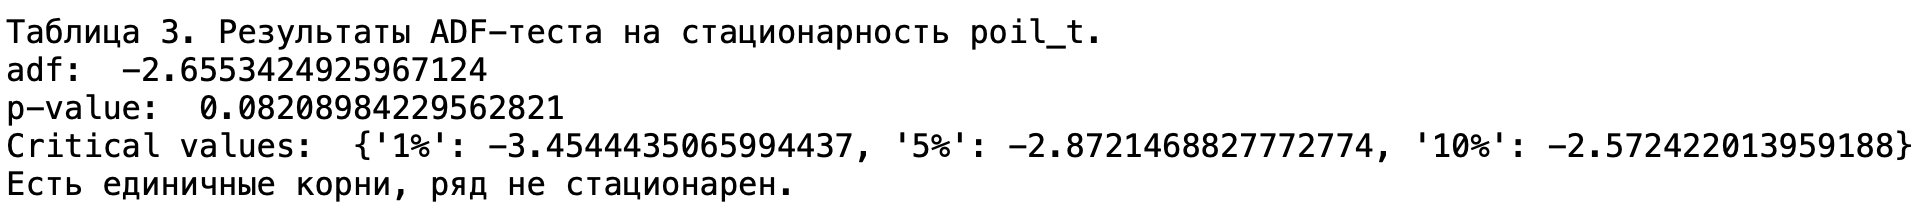
\includegraphics[width=150mm]{table_adf_poil.png}
\end{center}

\item ADF-тест на стационарность продифференциированного ряда 
$\Delta poil_t$:
\begin{center}
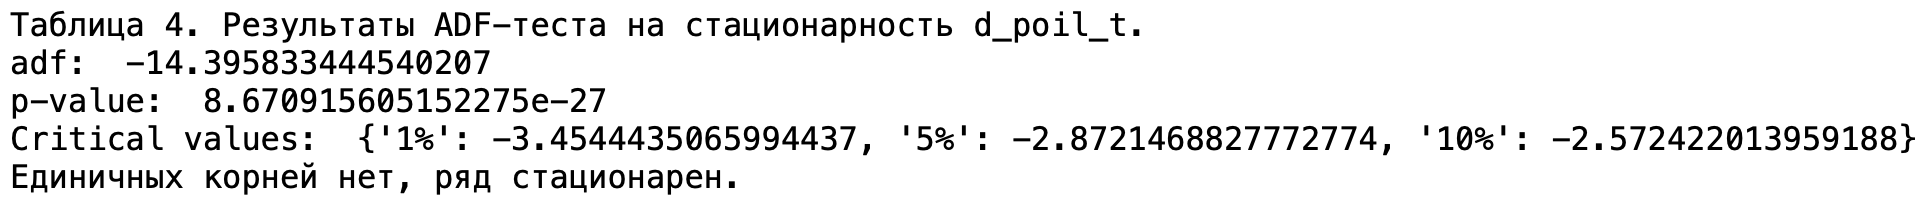
\includegraphics[width=150mm]{table_adf_dpoil.png}
\end{center}
\end{enumerate}
Таким образом, на уровне значимости $1\%$ получаем, что:
$$reer_t\nsim I(0),~reer_t\sim I(1),~poil_t\nsim I(0),~poil_t\sim I(1),$$
то есть гипотеза верна и $reer_t$ и $poil_t$ имеют единичные корни.

Теперь проверим с помощью того же ADF-теста временные ряды $log(reer_t)$ и $log(poil_t)$ на коинтегрированность. Для этого, используя МНК, оценим коэффициент $b$ в следующей регрессии:
$$log(reer_t)-b/cdot log(poil_t),$$
после чего проверим данный временной ряд(при найденном коэффициенте $b$) на стационарность.

ADF-тест на стационарность ряда $log(reer_t)-b\cdot log(poil_t)$:
\begin{center}
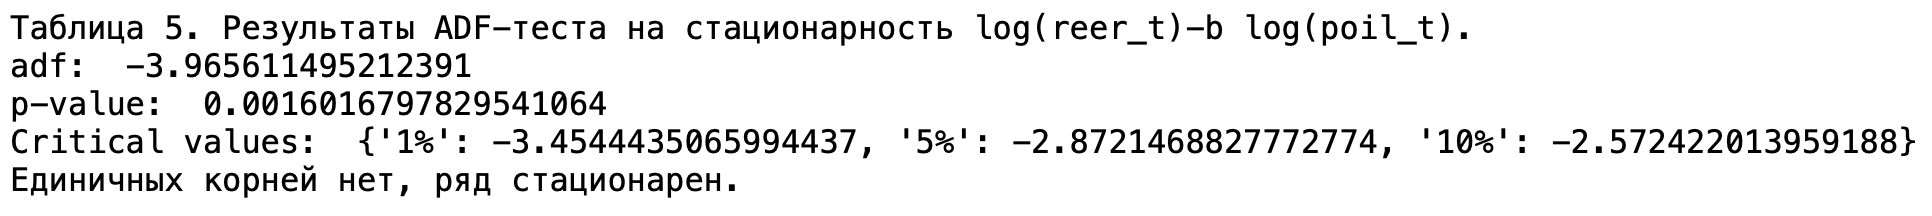
\includegraphics[width=150mm]{table_adf.png}
\end{center}
Таким образом, на уровне значимости $1\%$ получаем, что временной ряд $log(reer_t)-b\cdot log(poil_t)$  стационарен, то есть ряды $log(reer_t)$ и $log(poil_t)$ коинтегрированы.

\subsection{}
Так как в предыдущем пункте мы получили, что временные ряды$log(reer)_t\sim I(1)$ и $log(poil)_t\sim I(1)$ коинтегрированы, то из теории, описанной в \textbf{разделе 3}, то к ним применим метод \textbf{ECM}:
$$\Delta log(reer)_t=c_1+c_2z_{t-1}+\sum_{i=0}^p{a_i\cdot \Delta log(poil)_{t-i}}+\sum_{j=1}^q{b_i \cdot \Delta log(reer)_{t-j}}+\varepsilon_t,$$
где величина $z_t=(log(reer)_t-b\cdot log(poil)_t-E(log(reer)_t-b\cdot log(poil)_t))\sim I(0)$.

Однако согласно работе Лукаса (Lucas, 1976) при изменении экономической политики динамические взаимосвязи между макроэкономическими показателями также могут измениться. Это обусловлено тем, что динамика макроэкономической системы является результатом взаимодействия экономических агентов, которые при принятии решений учитывают изменения в экономической политике. В \textbf{разделе 2} мы уже перечисляли моменты смены экономической политики России, для построения модели выделим 1 наиболее значимое изменение: ноябрь 2014 года(переход к плавающему обменному курсу и таргетированию инфляции). Для каждого из 2-х получившихся периодов будет построена отдельная модель связи. Итого получаем модель:

\begin{equation*}
log(reer_t)=
 \begin{cases}
   \Delta log(reer)_t=c^1_1+c^1_2z_{t-1}+\sum_{i=0}^p{a^1_i\cdot \Delta log(poil)_{t-i}}+\sum_{j=1}^q{b^1_i \cdot \Delta log(reer)_{t-j}}+\varepsilon^1_t,~t<2014M11
   \\
   \Delta log(reer)_t=c^2_1+c^2_2z_{t-1}+\sum_{i=0}^p{a^2_i\cdot \Delta log(poil)_{t-i}}+\sum_{j=1}^q{b^2_i \cdot \Delta log(reer)_{t-j}}+\varepsilon^2_t,~t\geq 2014M11
 \end{cases}
\end{equation*}

Оценивать коэффициенты для данной модели будем следующим образом: вначале посчитаем величину $b$ линейной связи величин $log(reer)_t$ и $log(poil)_t$(было посчитано с помощью МНК в \textbf{5.1.4}), затем отдельно для каждой из 2 подзадач будем варьировать параметры количества запаздывающих членов $p$ и $q$ от $0$ до $6$(будем считать, что полугода измерений в худшем случае хватит), при каждых $(p,q)$ будем получать коэффициенты $c,~a_i,~b_j$ с помощью МНК(обычного метода наименьших квадратов), и по итогу для каждого интервала будем выбирать лучшую по качеству модель. Результаты оценки указаны в \textbf{таблицах 6,7}.

\begin{center}
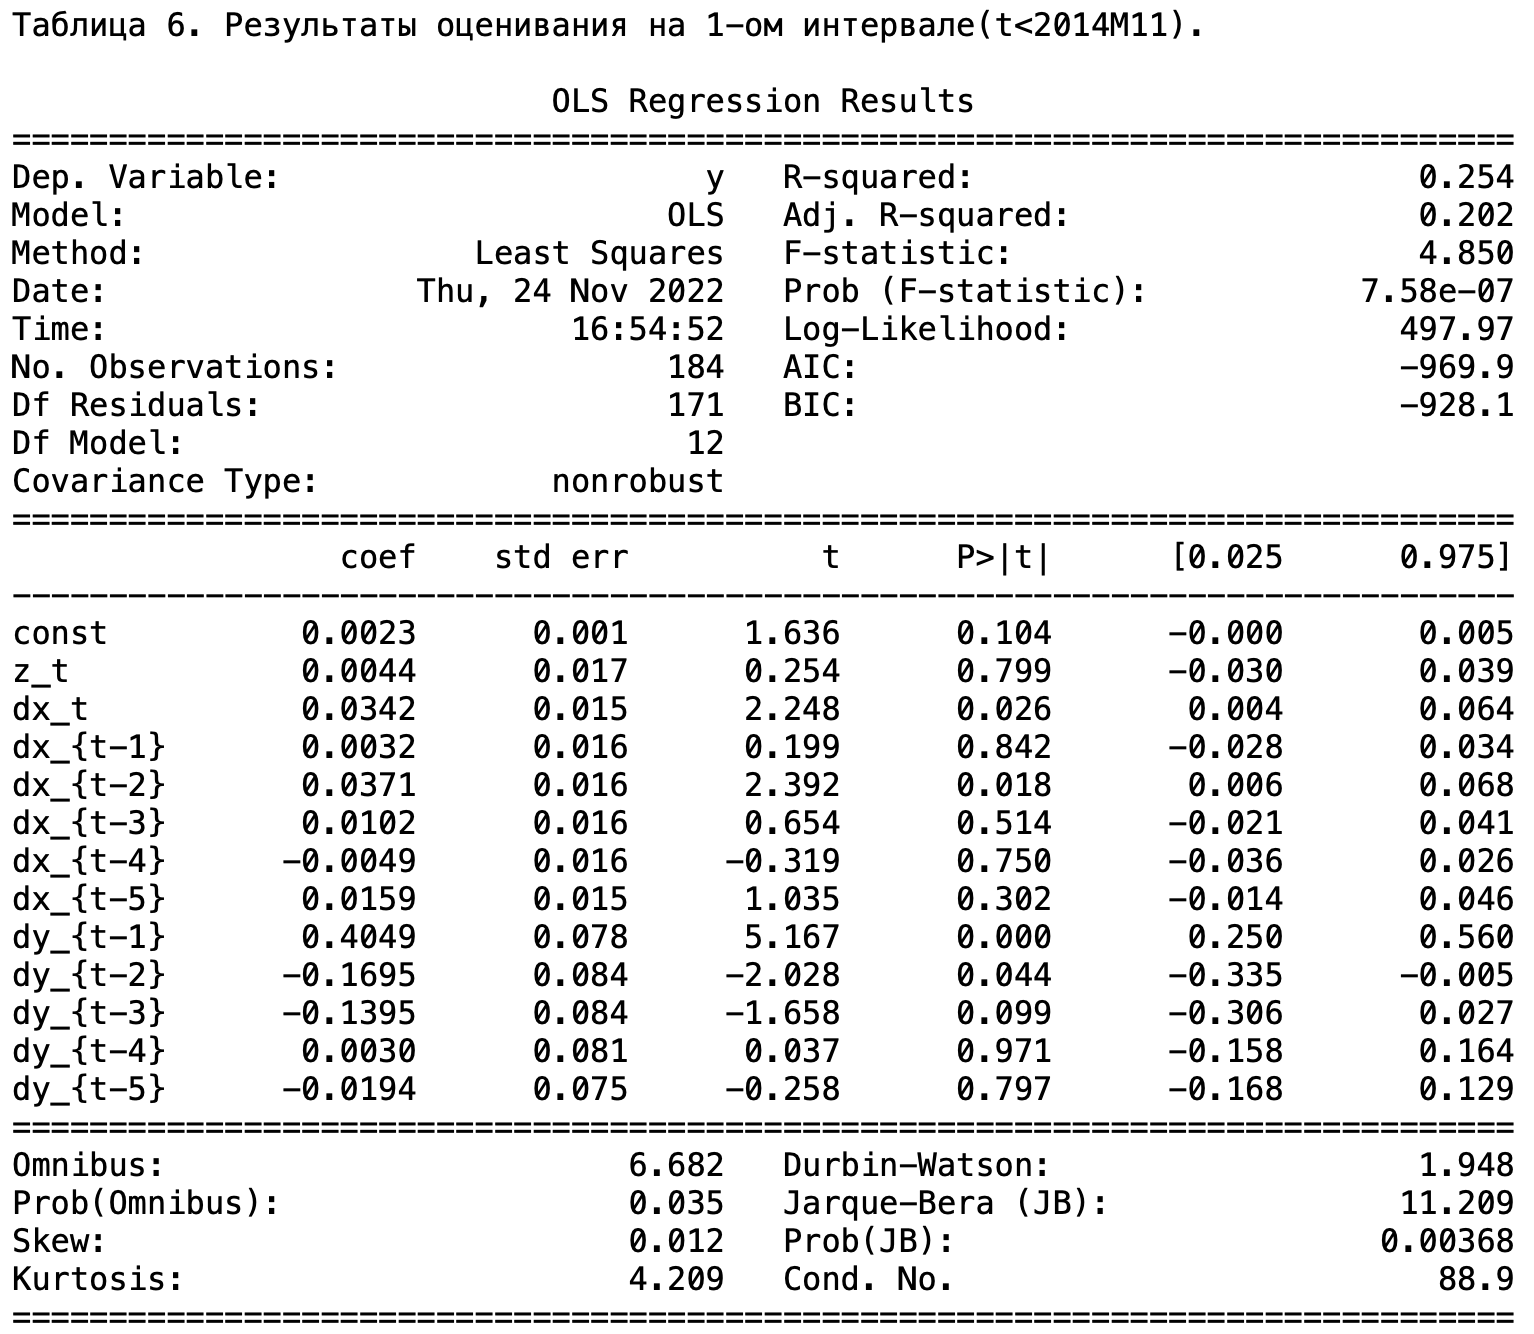
\includegraphics[width=150mm]{table6.png}
\end{center}

\begin{center}
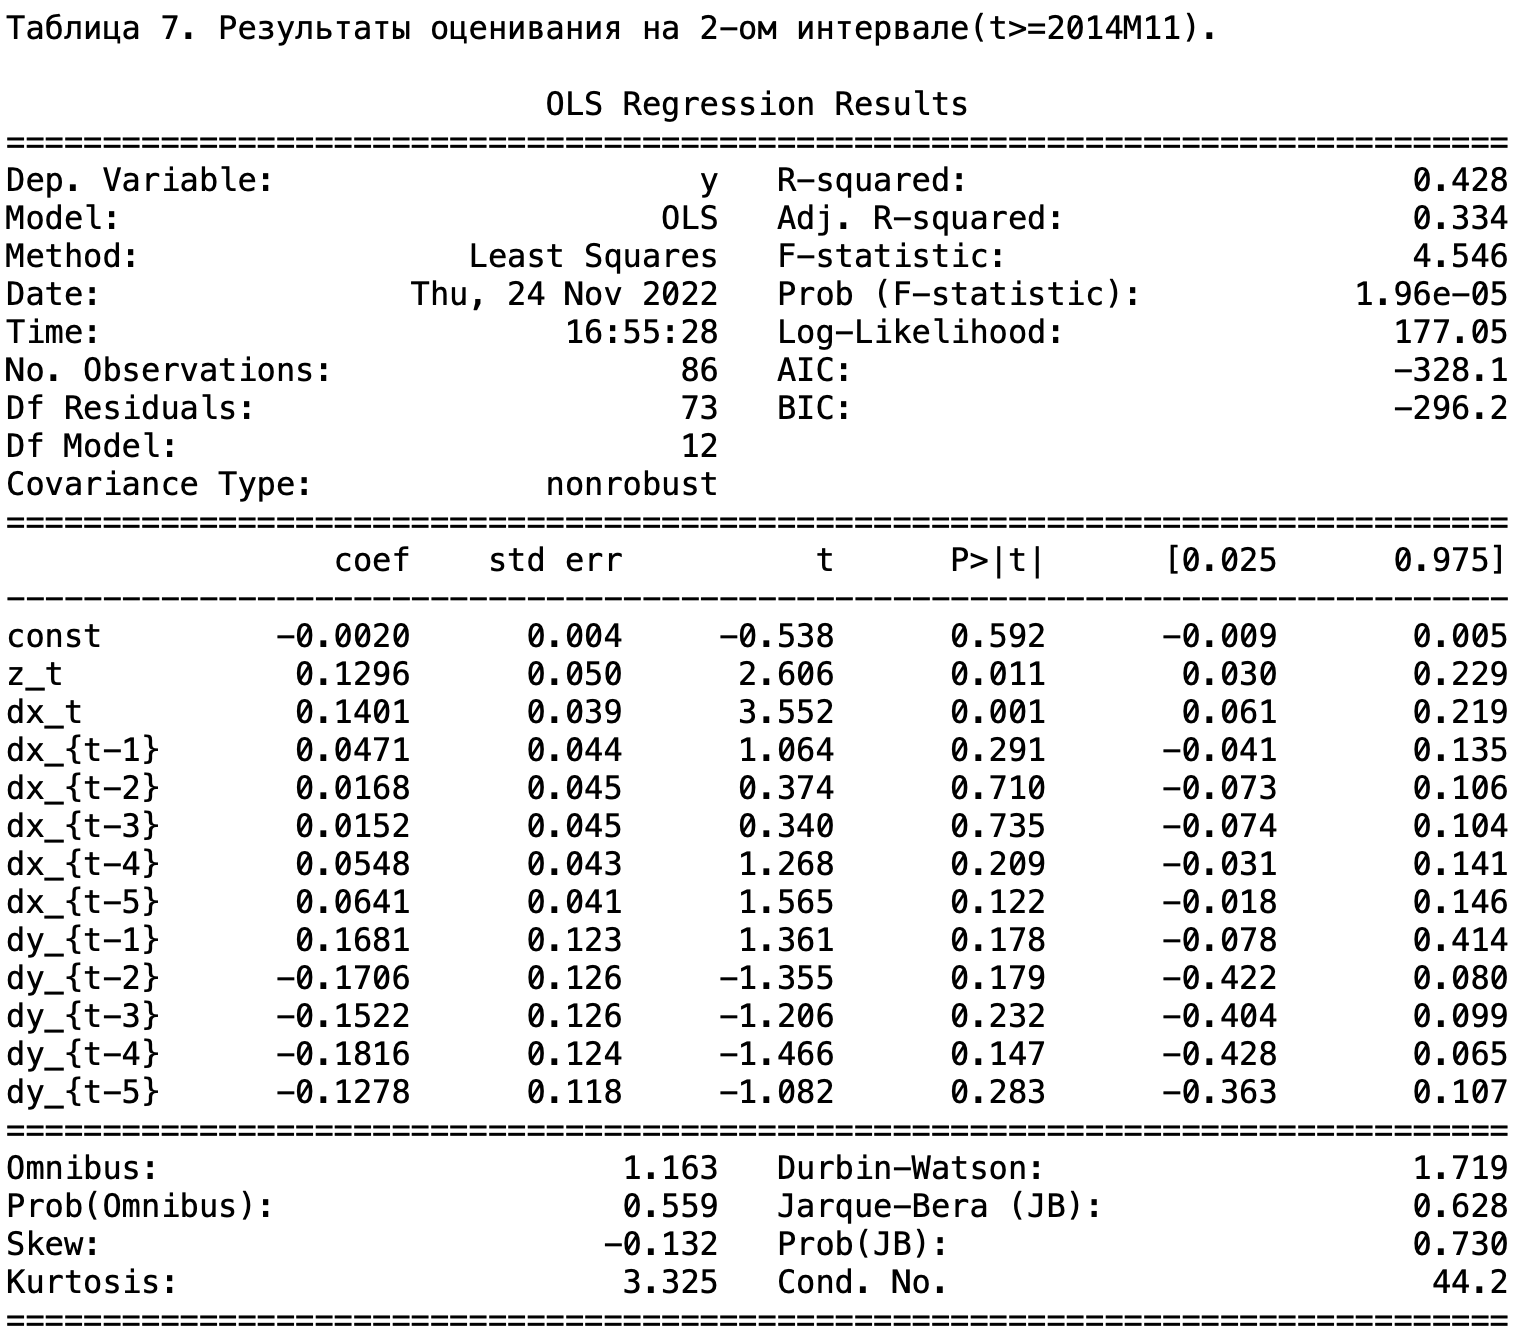
\includegraphics[width=150mm]{table7.png}
\end{center}

Из таблиц выше можно сделать несколько выводов, основанных на полученных коэффициентах регрессии:
\begin{enumerate}
\item Коэффициент при члене $z_t$(отклонение от долгосрочной связи) для 2-ой модели($t\geq 2014M11$) оказался на порядок выше коэффициента для 1-ой модели. Это означает, что 2-ая модель намного легче отклоняется от долгосрочной зависимости и сильнее зависит от краткосрочных скачков.
\item В то время как для 1-ой модели сильно превалируют коэффициенты авторегрессии, у 2-ой модели присутсвует довольно значительная связь $\Delta log(reer)_t$ и $\Delta log(poil)_t$ (коэффициент при $dx_t$ для 2-ой модели равен $0.1401$, что на порядок выше коэффициента для 1-ой модели).
\end{enumerate}

В заключение, построим график предсказания нашей модели, для наглядности на этом же графике изобразим и реальный временной ряд $log(reer)_t$. Результаты изображены на \textbf{рис. 4}.

\begin{center}
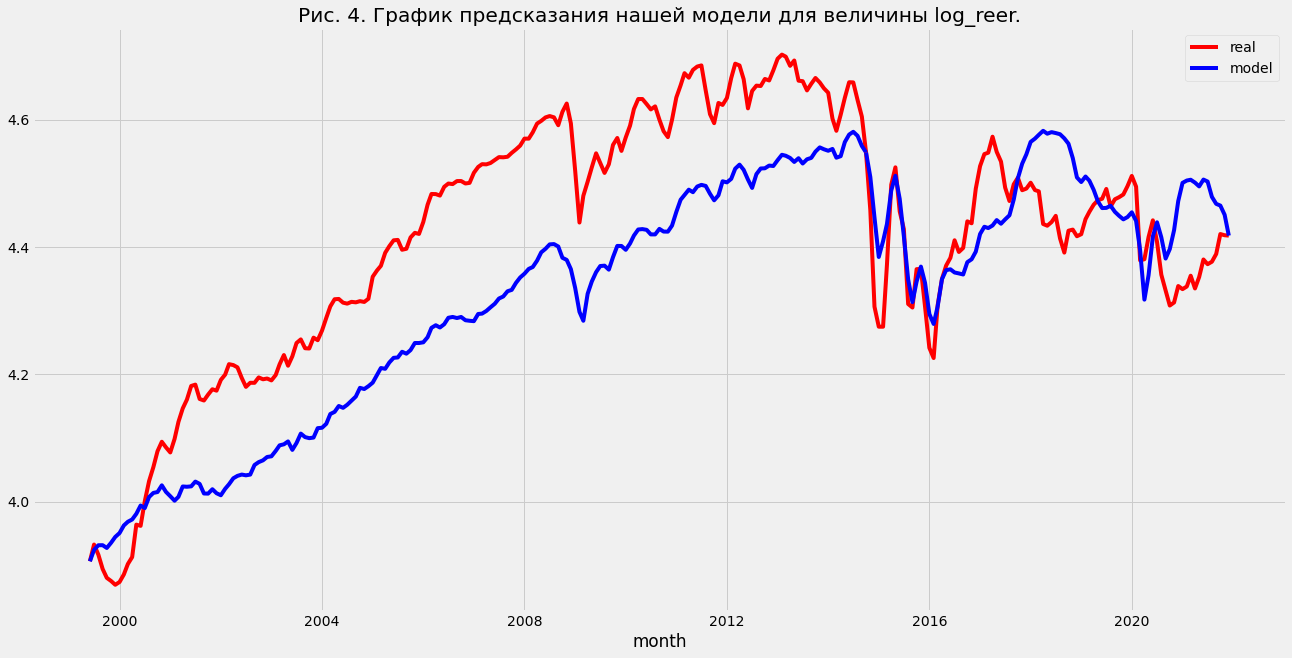
\includegraphics[width=150mm]{model_log_reer.png}
\end{center}

\section{Заключение}
В данной работе мы попытались построить модель связи реального эффективного обменного курса рубля и цены на нефть. В результате получились довольно качественные модели связи, однако они все еще довольно далеки от реальности. Основной проблемой оказались частые изменения денежно-кредитной политики России, ведь как показал анализ(построение 2-х разных моделей для 2-х промежутков времени, разделенных наиболее ярким изменением ДКП), с изменением ДКП изменяются и коэффициенты связи, причем в основном меняются именно коэффициенты короткосрочной связи(коэффициенты при переменной отклонения от долгосрочной связи). Возможно, стоит задуматься о построении более сложных моделей, учитывающих одновременно несколько детерминант. Однако целью данной работы было все же именно выявление связи между реальным эффективным обменным курсом и одной детерминантой(в нашем случае это цена на нефть), и эта цель была успешно выполнена.
\section{Литература}
А.В. Полбин (2017). Моделирование реального курса рубля в условиях изменения режима денежно-кредитной политики.

А. В. Полбин, А. В. Шумилов, А. Ф. Бедин, А. В. Куликов (2019). Модель реального обменного курса рубля с марковскими переключениями режимов.

В.П. Носко (2002). Введение в регрессионный анализ временных рядов.


\end{document}
